\scanpage{205}
% archive sheet number: 204

\[
 \begin{aligned}
 &\text{\textcircled{4}}+\text{\textcircled{4}}\\[-2pt]
 &\quad+\text{\textcircled{6}}
 \end{aligned}
 \ \boxed{\begin{matrix}\text{\textcircled{$b_s$}}&\text{\textcircled{$c_s$}}\\
 \multicolumn{2}{c}{\text{\textcircled{$t_a$}}}\end{matrix}}
 \quad\begin{aligned}&(s\in S)\\ &(a\in A)\end{aligned}
 \qquad \text{avec}\quad b_s=b_{\bar s},\ c_s=c_{\bar s},\ b_a=t_{\bar a}
\]

\figure{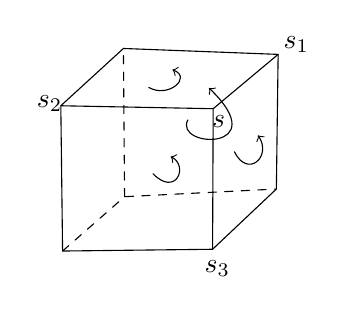
\begin{tikzpicture}[scale=.75,line cap=round]
\draw (0,0)--(2.54,.03)--(3.62,1.05)--(3.65,3.33)--(1.03,3.43)--(-.03,2.46)--(0,0);
\draw (-.03,2.46)--(2.55,2.41)--(3.65,3.33) (2.55,2.41)--(2.54,.03);
\draw[dashed] (0,0)--(1.05,.92)--(3.62,1.05) (1.05,.92)--(1.03,3.43);
\draw[->] (1.46,2.77) .. controls (1.79,2.58) and (2.20,2.94) .. (1.86,3.07);
\draw[->] (1.53,1.31) .. controls (1.92,.91) and (2.14,1.44) .. (1.83,1.60);
\draw[->] (2.91,1.68) .. controls (3.13,1.23) and (3.55,1.59) .. (3.31,1.96);
\draw[->] (2.12,2.22) .. controls (1.88,1.74) and (3.6,1.68) .. (2.48,2.76);
\node at (3.96,3.49) {$s_1$};\node at (-.22,2.5) {$s_2$};\node at (2.62,-.29) {$s_3$};\node at (2.64,2.20) {$s$};
\end{tikzpicture}}

Si $\delta(s)\inserted{\in I}$ est la diagonale qui passe par $s$, on a

\[
 \begin{aligned}b_s&=\operatorname{Tr}X_s\\c_s&=\det X_s\end{aligned}
\]

Si $\delta(a)\in\unsure{\mathcal P|P|\mathfrak P}_2(I)$ est \unsure{l'ens. des|l'une des} deux diagonales qui passent par les extr. de $a$, on a

\[
 \text{''}\qquad t_a=\operatorname{Tr}X_iX_j\inserted{=\operatorname{Tr}X_jX_i}
 \quad\text{si }\delta(a)=\{i,j\}
\]

\[
 4+4+\text{\textcircled{8}}\quad
 \underset{(s\in S)}{\boxed{\sigma_s,\pi_s,\text{\textcircled{$\unsure{T|\mathscr T|\tau|\mathbb T}_s$}}}}
\]

$s$ correspond \unsure{à|:} un triple $(i,j,\unsure{k|h})$ \unsure{à|:} perm. circulaire près

\[
 \begin{aligned}
 T_s&=\operatorname{Tr}X_iX_jX_k=\operatorname{Tr}X_{\deleted{\unsure{j}}j}X_kX_i=\operatorname{Tr}X_kX_iX_j\\
 T_{\bar s}&=\operatorname{Tr}X_kX_jX_i=\operatorname{Tr}X_jX_iX_k=\operatorname{Tr}X_iX_kX_j
 \end{aligned}
\]

\tikz[baseline=(a.base)]\node[draw,ellipse,inner sep=2pt] (a) {$4+4$ relations}; $\left(\begin{smallmatrix} R_s\\\wr\\R_{\bar s}\end{smallmatrix}\right)$

\[
 \boxed{\begin{aligned}
 \sigma_s&=\sigma_{\bar s}=T_s+T_{\bar s}\\
 \pi_s&=\pi_{\bar s}=T_s\cdot T_{\bar s}
 \end{aligned}}
\]

\[
 \begin{aligned}
 \sigma_s=\sigma_{\bar s}&=b_it_{jk}+b_jt_{ki}+b_kt_{ij}-b_ib_jb_k\\
 \deleted{\unsure{R_s=}}&=b_{s_1}t_{ss_1}+b_{s_2}t_{ss_2}+b_{s_3}t_{ss_3}-b_{s_1}b_{s_2}b_{s_3}
 \end{aligned}
\]

où $s_1,s_2,s_3$ sont les sommets adjacents à $s$

\[
 \begin{aligned}
 \unsure{\Pi|\pi}_s=\Pi_{\bar s}={}&t_{ss_1}t_{ss_2}t_{ss_3}
 +\deleted{(c_{s_1}t_{ss_1}+c_{s_2}t_{ss_2}+c_{s_3}t_{ss_3})}\\
 &\inserted{\bigl[c_{s_1}t_{ss_1}(t_{ss_1}-b_{s_2}b_{s_3})+
 c_{s_2}t_{ss_2}(t_{ss_2}-b_{s_3}b_{s_1})+
 c_{s_3}t_{ss_3}(\unsure{t_{s_3s_3}|t_{ss_3}|t_{s_1s_2}}-b_{s_1}b_{s_2})\bigr]}\\
 &+(b_{ss_1}^{2}c_{ss_2}c_{ss_3}+b_{ss_2}^{2}c_{ss_3}c_{ss_1}+b_{ss_3}^{2}c_{ss_1}c_{ss_2})
 \end{aligned}
\]

\[
 \text{\textcircled{6}}\quad
 \begin{array}{|c@{\ }l}\cline{1-1}
 \text{\textcircled{$T_f$}}\vrule & (f\in F)\\ \cline{2-2}
 \multicolumn{2}{|c|}{\sigma_a,\pi_a}\\\hline\end{array}\quad (a\in A)
\]

Si $f$ correspond à la permutation circulaire $(i,j,k,\unsure{l|\ell|e})$ de $I$, on a

\[
 T_f=\operatorname{Tr}X_iX_jX_kX_l=\deleted{\unsure{t_f=|\mathbb T_f=}}\operatorname{Tr}X_jX_kX_lX_i
 =\operatorname{Tr}X_kX_lX_iX_j=\operatorname{Tr}X_lX_iX_jX_k
\]

Si $f,f'$ sont adjacentes le long d'une arête $a=(s,t)$

\figure{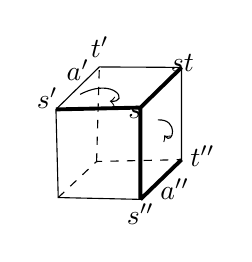
\begin{tikzpicture}[scale=.58]
\draw (0,0)--(1.8,-.04)--(2.7,.83)--(2.7,2.85)--(.90,2.86)--(-.05,1.93)--cycle;
\draw[line width=1.4pt] (-.05,1.93)--(1.8,1.97)--(2.7,2.85) (1.8,1.97)--(1.8,-.04) (1.8,-.04)--(2.7,.83);
\draw[dashed] (0,0)--(.84,.79)--(2.7,.83) (.84,.79)--(.90,2.86);
\draw[->] (.48,2.26) .. controls (1.23,2.65) and (1.57,2.08) .. (1.13,2.11);
\draw[->] (2.18,1.70) .. controls (2.65,1.73) and (2.52,1.13) .. (2.32,1.36);
\node at (-.24,2.18) {$s'$};\node at (.43,2.78) {$a'$};\node at (.91,3.29) {$t'$};\node at (2.72,2.95) {$\deleted{\unsure{s}}t$};
\node at (1.68,1.86) {$s$};\node at (1.8,-.37) {$s''$};\node at (2.55,.18) {$a''$};\node at (3.16,.91) {$t''$};
\end{tikzpicture}}

\diagram{\begin{tikzcd}[ampersand replacement=\&,column sep=1pt,row sep=3pt]
 f=(s\arrow[d]\&{,}t\arrow[d]\&{,}s'\arrow[d]\&{,}t')\arrow[d]\&{,}\quad f'=(t\arrow[d]\&{,}s\arrow[d]\&{,}t''\arrow[d]\&{,}s'')\arrow[d]\\
 i\&j\&k\&l\&j\&i\&k\&l
\end{tikzcd}}

\deleted{\unsure{Nb}} d'où $T_f=\operatorname{Tr}X_iX_j(X_kX_l)$, $T_{f'}=\operatorname{Tr}X_jX_i(X_kX_l)$, on a
